\subsection{Context Manager}
\label{sec:context-manager}

\begin{figure}
  \centering
  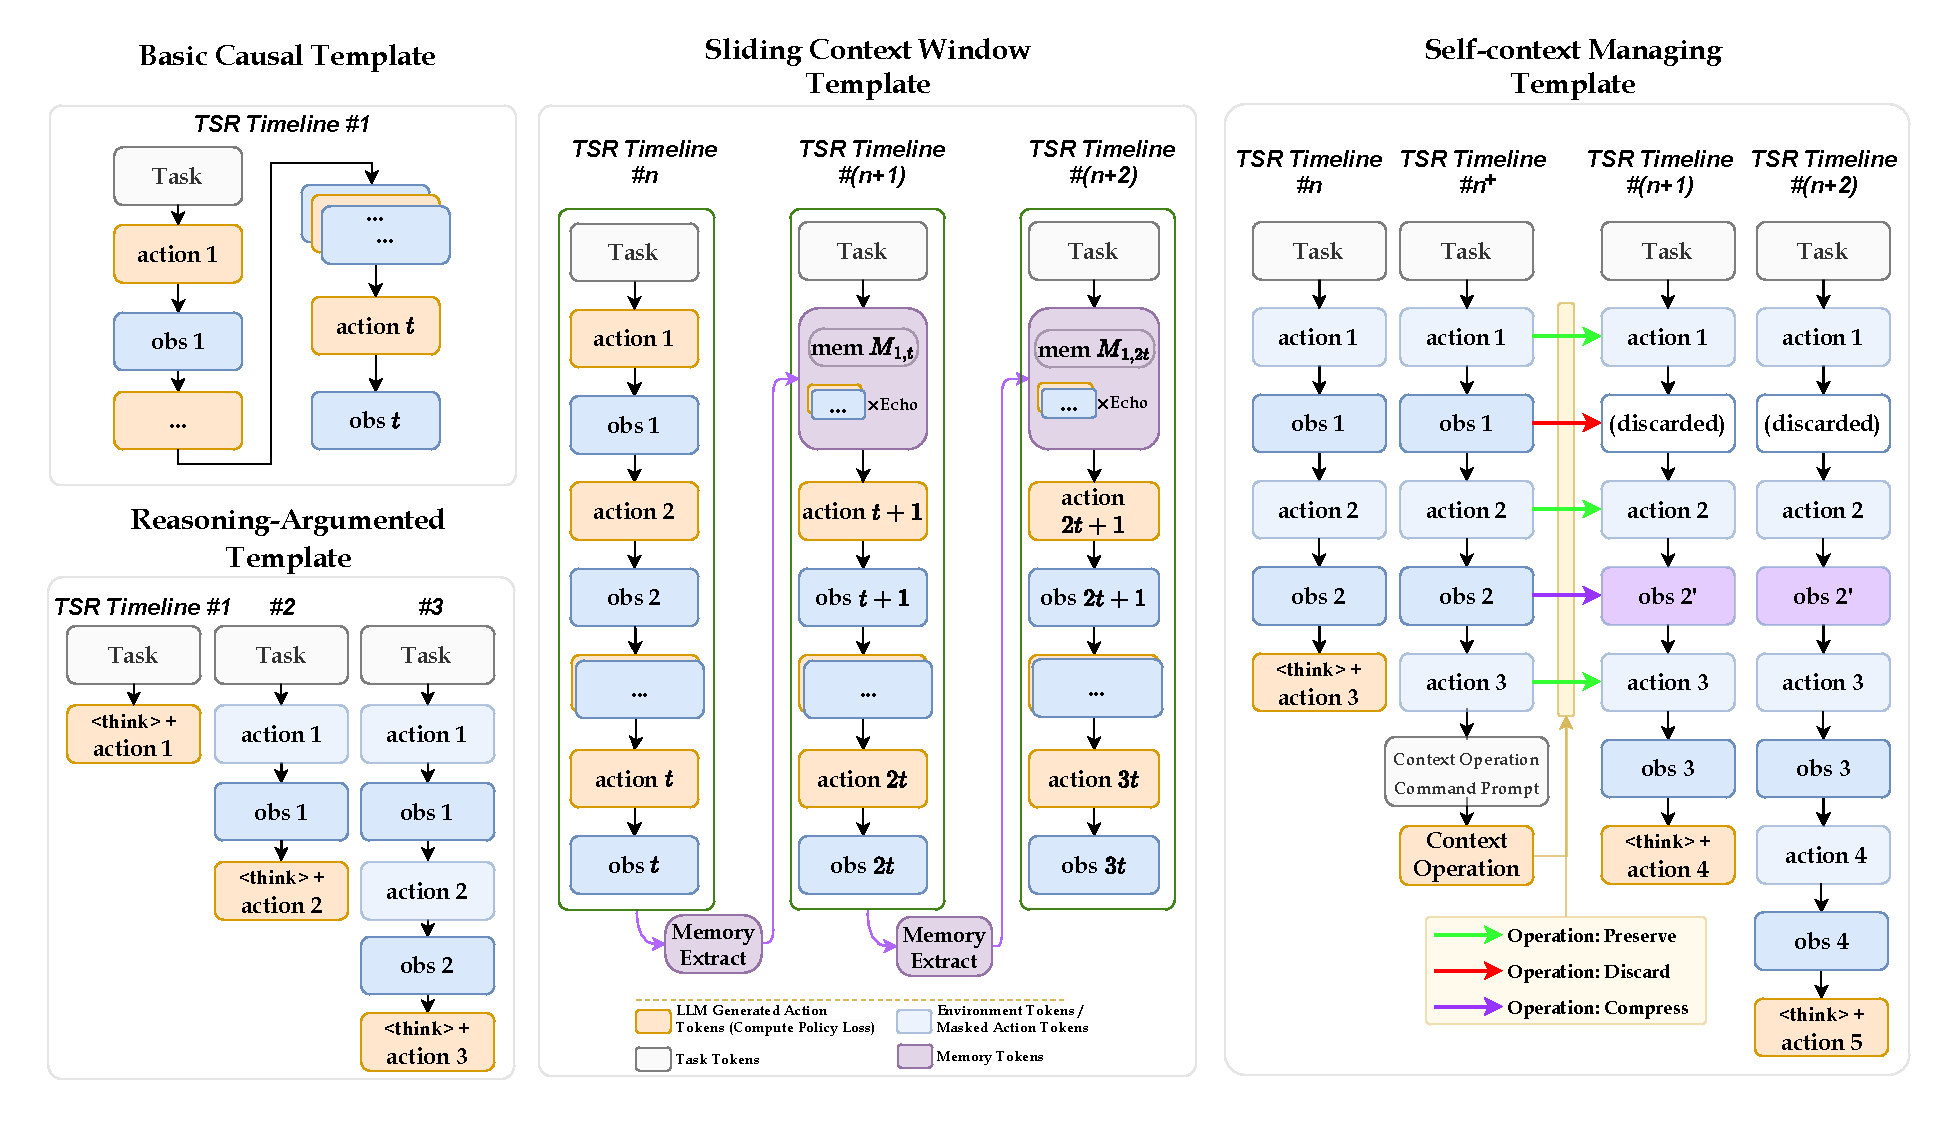
\includegraphics[width=1.0\textwidth]{figs/cmt_basic_four_4.drawio_new.pdf}
  \caption{The four fundamental context managing templates of AgentEvolver. Yellow blocks indicate LLM messages, blue blocks correspond to environment messages or messages masked from loss function, and purple blocks represent memory messages. The displayed timelines depict the anticipated outcomes after the Timeline Snapshot Recorder (TSR) completes the timeline merging process.}
  \label{fig:cmts}
\end{figure}


Long-horizon reinforcement learning with large language models (LLMs) requires not only reasoning and planning, but also dynamic management of historical context across multiple interactions. 
Existing paradigms exhibit a trade-off: the \emph{causal multi-step rollout} paradigm maintains strong temporal consistency but lacks flexibility~\citep{jin2025search}, while the \emph{step-independent multi-turn rollout} paradigm offers full editability at the cost of significant computational overhead~\citep{feng2025group}. 
To unify these two perspectives, AgentEvolver introduces a \textbf{Context Manager (CM)} that serves as the central infrastructure for controlling context evolution during agent–environment interactions.

The CM provides a consistent interface for both causal and non-causal interaction modes, enabling efficient, adaptive, and reasoning-aware rollouts. 
Its design aims to (1) maintain the computational efficiency of causal training, (2) allow selective modification of historical context when necessary, and (3) support agents that can eventually \emph{self-manage} their own context. 
To achieve this, CM introduces two fundamental data structures shared across all rollout paradigms.

\paragraph{Core Abstractions: Live Timeline and Snapshot Recorder.}
The Context Manager operates on two simple yet powerful primitives:
\begin{itemize}
    \item \textbf{Live Context Timeline (LCT)} — a mutable sequence representing the agent’s current working context during multi-turn interaction.
    \item \textbf{Timeline Snapshot Recorder (TSR)} — an immutable buffer that stores frozen snapshots of the LCT whenever the policy LLM generates an action.
\end{itemize}

The LCT acts as the agent’s short-term, editable memory, while the TSR maintains a verifiable, token-level record of the entire episode. 
After each rollout, the TSR automatically performs \emph{timeline merging}, removing redundant subsequences and aligning loss masks across overlapping segments. 
This dual-structure design allows CM to support both efficient causal rollouts and flexible reasoning-oriented rollouts within a unified framework.

\subsubsection{Rollout Paradigms and Context-Managing Templates}
\label{sec:cmt}

Built upon the LCT–TSR abstraction, the Context Manager defines a family of \textbf{Context-Managing Templates (CMTs)}. 
Each template specifies how the LCT evolves during interaction, thus representing a different balance between efficiency, reasoning capacity, and autonomy. 
The four fundamental templates are illustrated in Figure~\ref{fig:cmts}.

\paragraph{(i) Basic Causal Template — Efficient and Deterministic.}
The simplest template follows a strictly causal organization of messages. 
At the beginning of an episode, the initial task instruction is appended to the LCT. 
The agent then repeats the observe–act cycle until termination, after which only the final LCT snapshot is retained by the TSR.
This design ensures full temporal consistency and low computational cost, making it ideal for search-style RL training~\citep{jin2025search}. 
However, since messages cannot be edited or removed, memory consumption grows linearly with context length, and the lack of editability complicates reasoning-intensive behaviors.

\paragraph{(ii) Reasoning-Augmented Template — Structured Thinking Before Action.}
Reasoning before action has proven beneficial in complex decision-making tasks~\citep{guo2025deepseek}. 
The reasoning-augmented template trains agents to explicitly \emph{think before acting}. 
For models without pre-trained reasoning ability (e.g., Qwen2~\citep{team2024qwen2}), structured prompts encourage the model to generate \texttt{<think>} tokens before decisions, with additional rewards promoting high-quality reasoning. 
For models that already possess reasoning skills (e.g., Qwen3-14B~\citep{qwen2025technical}), the template enhances consistency and efficiency. 

\paragraph{(iii) Sliding Context Window Template — Scalable to Long Horizons.}
Long-horizon tasks often generate hundreds or thousands of interaction steps, exceeding the token capacity of typical LLMs. 
To address this, the sliding context window template treats the LCT as a moving window. 
When its size exceeds a predefined threshold, the Context Manager summarizes older content into a compressed \textit{memory message} and initializes a new timeline window for subsequent interactions. 
After timeline merging, only a minimal set of window snapshots remains. 
This approach preserves local causality while keeping GPU memory usage constant, achieving scalability to arbitrarily long episodes.

\paragraph{(iv) Self-Context Managing Template — Toward Autonomy.}
The previous templates rely on fixed rules for context updates. 
In contrast, the self-context managing template allows the agent to \emph{actively control} its own memory. 
When the LCT exceeds a token limit, the CM triggers a special \textit{context operation prompt}, asking the policy LLM to select for each message one of three operations:
\[
a_\text{context} \in \{\alpha_\text{keep}, \alpha_\text{remove}, \alpha_\text{compress}\},
\]
corresponding to preservation, deletion, and compression (via an external summarizing LLM).
This paradigm enables fine-grained control over the token budget and encourages the emergence of self-regulated information filtering behavior. 
It is particularly effective in environments that generate large amounts of uninformative text.

\paragraph{Discussion.}
All four templates share the same underlying LCT–TSR mechanism but differ in how they manipulate or delegate control over context evolution. 
Together, they form a spectrum from rigid causality to full autonomy: the Basic Causal Template maximizes efficiency, while the Self-Context Managing Template empowers agents to regulate their own memory dynamically. 
This unified view of context management provides a principled foundation for building scalable, reasoning-capable, and self-adaptive LLM agents.
